% Created by tikzDevice version 0.12.6 on 2024-11-10 08:14:27
% !TEX encoding = UTF-8 Unicode
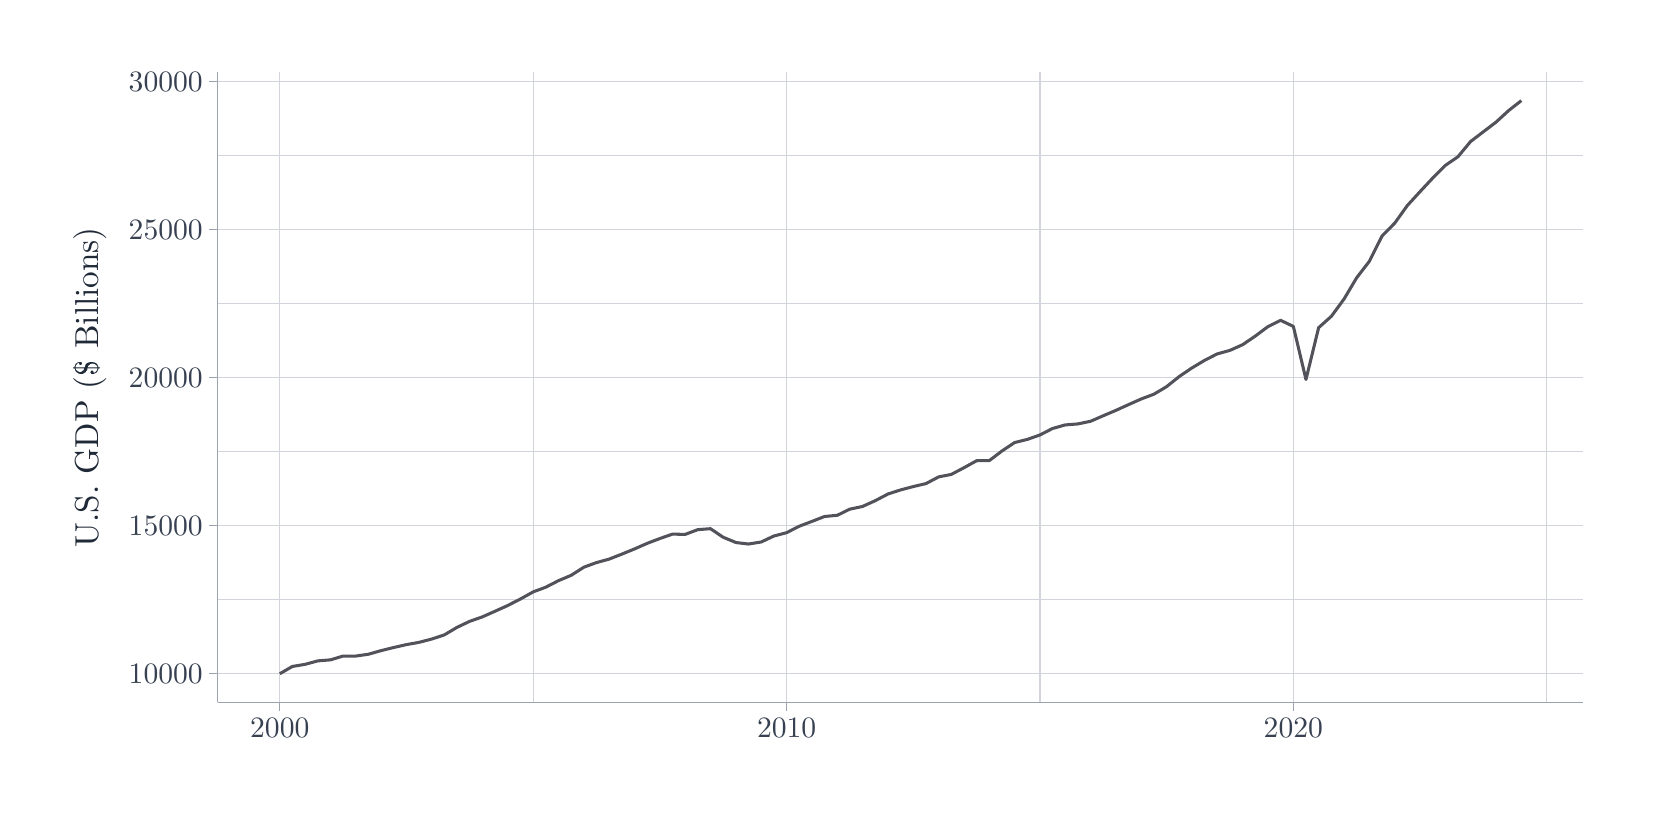
\begin{tikzpicture}[x=1pt,y=1pt]
\definecolor{fillColor}{RGB}{255,255,255}
\path[use as bounding box,fill=fillColor] (0,0) rectangle (578.16,274.63);
\begin{scope}
\path[clip] (  0.00,  0.00) rectangle (578.16,274.63);
\definecolor{drawColor}{RGB}{255,255,255}

\path[draw=drawColor,line width= 0.6pt,line join=round,line cap=round,fill=fillColor] ( -0.00,  0.00) rectangle (578.16,274.63);
\end{scope}
\begin{scope}
\path[clip] ( 68.67, 30.82) rectangle (562.16,258.63);
\definecolor{drawColor}{RGB}{255,255,255}
\definecolor{fillColor}{RGB}{255,255,255}

\path[draw=drawColor,line width= 0.6pt,line join=round,line cap=round,fill=fillColor] ( 68.67, 30.82) rectangle (562.16,258.63);
\definecolor{drawColor}{RGB}{209,213,219}

\path[draw=drawColor,line width= 0.4pt,line join=round] ( 68.67, 67.91) --
	(562.16, 67.91);

\path[draw=drawColor,line width= 0.4pt,line join=round] ( 68.67,121.43) --
	(562.16,121.43);

\path[draw=drawColor,line width= 0.4pt,line join=round] ( 68.67,174.95) --
	(562.16,174.95);

\path[draw=drawColor,line width= 0.4pt,line join=round] ( 68.67,228.47) --
	(562.16,228.47);

\path[draw=drawColor,line width= 0.4pt,line join=round] (182.67, 30.82) --
	(182.67,258.63);

\path[draw=drawColor,line width= 0.4pt,line join=round] (365.80, 30.82) --
	(365.80,258.63);

\path[draw=drawColor,line width= 0.4pt,line join=round] (548.93, 30.82) --
	(548.93,258.63);

\path[draw=drawColor,line width= 0.4pt,line join=round] ( 68.67, 41.15) --
	(562.16, 41.15);

\path[draw=drawColor,line width= 0.4pt,line join=round] ( 68.67, 94.67) --
	(562.16, 94.67);

\path[draw=drawColor,line width= 0.4pt,line join=round] ( 68.67,148.19) --
	(562.16,148.19);

\path[draw=drawColor,line width= 0.4pt,line join=round] ( 68.67,201.71) --
	(562.16,201.71);

\path[draw=drawColor,line width= 0.4pt,line join=round] ( 68.67,255.23) --
	(562.16,255.23);

\path[draw=drawColor,line width= 0.4pt,line join=round] ( 91.10, 30.82) --
	( 91.10,258.63);

\path[draw=drawColor,line width= 0.4pt,line join=round] (274.25, 30.82) --
	(274.25,258.63);

\path[draw=drawColor,line width= 0.4pt,line join=round] (457.35, 30.82) --
	(457.35,258.63);
\definecolor{drawColor}{RGB}{82,82,91}

\path[draw=drawColor,line width= 1.1pt,line join=round] ( 91.10, 41.18) --
	( 95.66, 43.81) --
	(100.22, 44.56) --
	(104.84, 45.82) --
	(109.45, 46.19) --
	(113.96, 47.57) --
	(118.52, 47.56) --
	(123.14, 48.22) --
	(127.75, 49.54) --
	(132.26, 50.65) --
	(136.82, 51.69) --
	(141.44, 52.52) --
	(146.05, 53.72) --
	(150.56, 55.21) --
	(155.12, 57.92) --
	(159.74, 60.12) --
	(164.35, 61.74) --
	(168.91, 63.77) --
	(173.47, 65.83) --
	(178.09, 68.20) --
	(182.70, 70.77) --
	(187.21, 72.44) --
	(191.77, 74.79) --
	(196.39, 76.74) --
	(201.00, 79.68) --
	(205.51, 81.33) --
	(210.07, 82.58) --
	(214.69, 84.39) --
	(219.30, 86.28) --
	(223.81, 88.27) --
	(228.37, 90.01) --
	(232.99, 91.62) --
	(237.60, 91.53) --
	(242.16, 93.24) --
	(246.72, 93.59) --
	(251.34, 90.48) --
	(255.95, 88.58) --
	(260.46, 88.05) --
	(265.02, 88.77) --
	(269.64, 90.94) --
	(274.25, 92.15) --
	(278.76, 94.46) --
	(283.32, 96.19) --
	(287.94, 97.99) --
	(292.55, 98.43) --
	(297.06,100.64) --
	(301.63,101.61) --
	(306.24,103.69) --
	(310.85,106.11) --
	(315.41,107.59) --
	(319.98,108.80) --
	(324.59,109.88) --
	(329.20,112.31) --
	(333.71,113.18) --
	(338.28,115.59) --
	(342.89,118.14) --
	(347.50,118.20) --
	(352.01,121.63) --
	(356.58,124.69) --
	(361.19,125.84) --
	(365.80,127.46) --
	(370.31,129.78) --
	(374.88,131.08) --
	(379.49,131.44) --
	(384.10,132.41) --
	(388.66,134.40) --
	(393.23,136.34) --
	(397.84,138.44) --
	(402.45,140.49) --
	(406.96,142.18) --
	(411.53,144.90) --
	(416.14,148.59) --
	(420.75,151.71) --
	(425.26,154.41) --
	(429.83,156.74) --
	(434.44,158.02) --
	(439.05,160.09) --
	(443.56,163.16) --
	(448.13,166.57) --
	(452.74,168.88) --
	(457.35,166.68) --
	(461.91,147.50) --
	(466.48,166.22) --
	(471.09,170.34) --
	(475.70,176.63) --
	(480.22,184.25) --
	(484.78,190.17) --
	(489.39,199.32) --
	(494.00,204.02) --
	(498.52,210.34) --
	(503.08,215.33) --
	(507.69,220.27) --
	(512.30,224.88) --
	(516.82,227.98) --
	(521.38,233.48) --
	(525.99,237.00) --
	(530.60,240.50) --
	(535.17,244.70) --
	(539.73,248.27);
\end{scope}
\begin{scope}
\path[clip] (  0.00,  0.00) rectangle (578.16,274.63);
\definecolor{drawColor}{RGB}{156,163,175}

\path[draw=drawColor,line width= 0.3pt,line join=round] ( 68.67, 30.82) --
	( 68.67,258.63);
\end{scope}
\begin{scope}
\path[clip] (  0.00,  0.00) rectangle (578.16,274.63);
\definecolor{drawColor}{RGB}{55,65,81}

\node[text=drawColor,anchor=base east,inner sep=0pt, outer sep=0pt, scale=  1.07] at ( 63.27, 37.48) {10000};

\node[text=drawColor,anchor=base east,inner sep=0pt, outer sep=0pt, scale=  1.07] at ( 63.27, 91.00) {15000};

\node[text=drawColor,anchor=base east,inner sep=0pt, outer sep=0pt, scale=  1.07] at ( 63.27,144.52) {20000};

\node[text=drawColor,anchor=base east,inner sep=0pt, outer sep=0pt, scale=  1.07] at ( 63.27,198.04) {25000};

\node[text=drawColor,anchor=base east,inner sep=0pt, outer sep=0pt, scale=  1.07] at ( 63.27,251.56) {30000};
\end{scope}
\begin{scope}
\path[clip] (  0.00,  0.00) rectangle (578.16,274.63);
\definecolor{drawColor}{RGB}{156,163,175}

\path[draw=drawColor,line width= 0.3pt,line join=round] ( 65.67, 41.15) --
	( 68.67, 41.15);

\path[draw=drawColor,line width= 0.3pt,line join=round] ( 65.67, 94.67) --
	( 68.67, 94.67);

\path[draw=drawColor,line width= 0.3pt,line join=round] ( 65.67,148.19) --
	( 68.67,148.19);

\path[draw=drawColor,line width= 0.3pt,line join=round] ( 65.67,201.71) --
	( 68.67,201.71);

\path[draw=drawColor,line width= 0.3pt,line join=round] ( 65.67,255.23) --
	( 68.67,255.23);
\end{scope}
\begin{scope}
\path[clip] (  0.00,  0.00) rectangle (578.16,274.63);
\definecolor{drawColor}{RGB}{156,163,175}

\path[draw=drawColor,line width= 0.3pt,line join=round] ( 68.67, 30.82) --
	(562.16, 30.82);
\end{scope}
\begin{scope}
\path[clip] (  0.00,  0.00) rectangle (578.16,274.63);
\definecolor{drawColor}{RGB}{156,163,175}

\path[draw=drawColor,line width= 0.3pt,line join=round] ( 91.10, 27.82) --
	( 91.10, 30.82);

\path[draw=drawColor,line width= 0.3pt,line join=round] (274.25, 27.82) --
	(274.25, 30.82);

\path[draw=drawColor,line width= 0.3pt,line join=round] (457.35, 27.82) --
	(457.35, 30.82);
\end{scope}
\begin{scope}
\path[clip] (  0.00,  0.00) rectangle (578.16,274.63);
\definecolor{drawColor}{RGB}{55,65,81}

\node[text=drawColor,anchor=base,inner sep=0pt, outer sep=0pt, scale=  1.07] at ( 91.10, 18.07) {2000};

\node[text=drawColor,anchor=base,inner sep=0pt, outer sep=0pt, scale=  1.07] at (274.25, 18.07) {2010};

\node[text=drawColor,anchor=base,inner sep=0pt, outer sep=0pt, scale=  1.07] at (457.35, 18.07) {2020};
\end{scope}
\begin{scope}
\path[clip] (  0.00,  0.00) rectangle (578.16,274.63);
\definecolor{drawColor}{RGB}{31,41,55}

\node[text=drawColor,rotate= 90.00,anchor=base,inner sep=0pt, outer sep=0pt, scale=  1.20] at ( 25.43,144.72) {U.S. GDP (\$ Billions)};
\end{scope}
\end{tikzpicture}
